%\section{Class Diagram}
\section{Component architecture}

The architecture of the administration part of the GIRAF system is designed as a client-server architecture. Which means that the user uses the client to communicate with the server, where database lies. Within the client and the server lie three components. These components are called; view, controller and database. These three components communicate with each other through the controller, meaning that controller is the link between the view and the database, which handles calls from both sides. In current design the client does not contain any components, leaving the server with all three, the reason is that the system is 100\% web based and is utilized by means of an internet browser. The componentarchitecture can be seen in figure \vref{fig:architecture}

\begin{figure}[!ht]
\centering
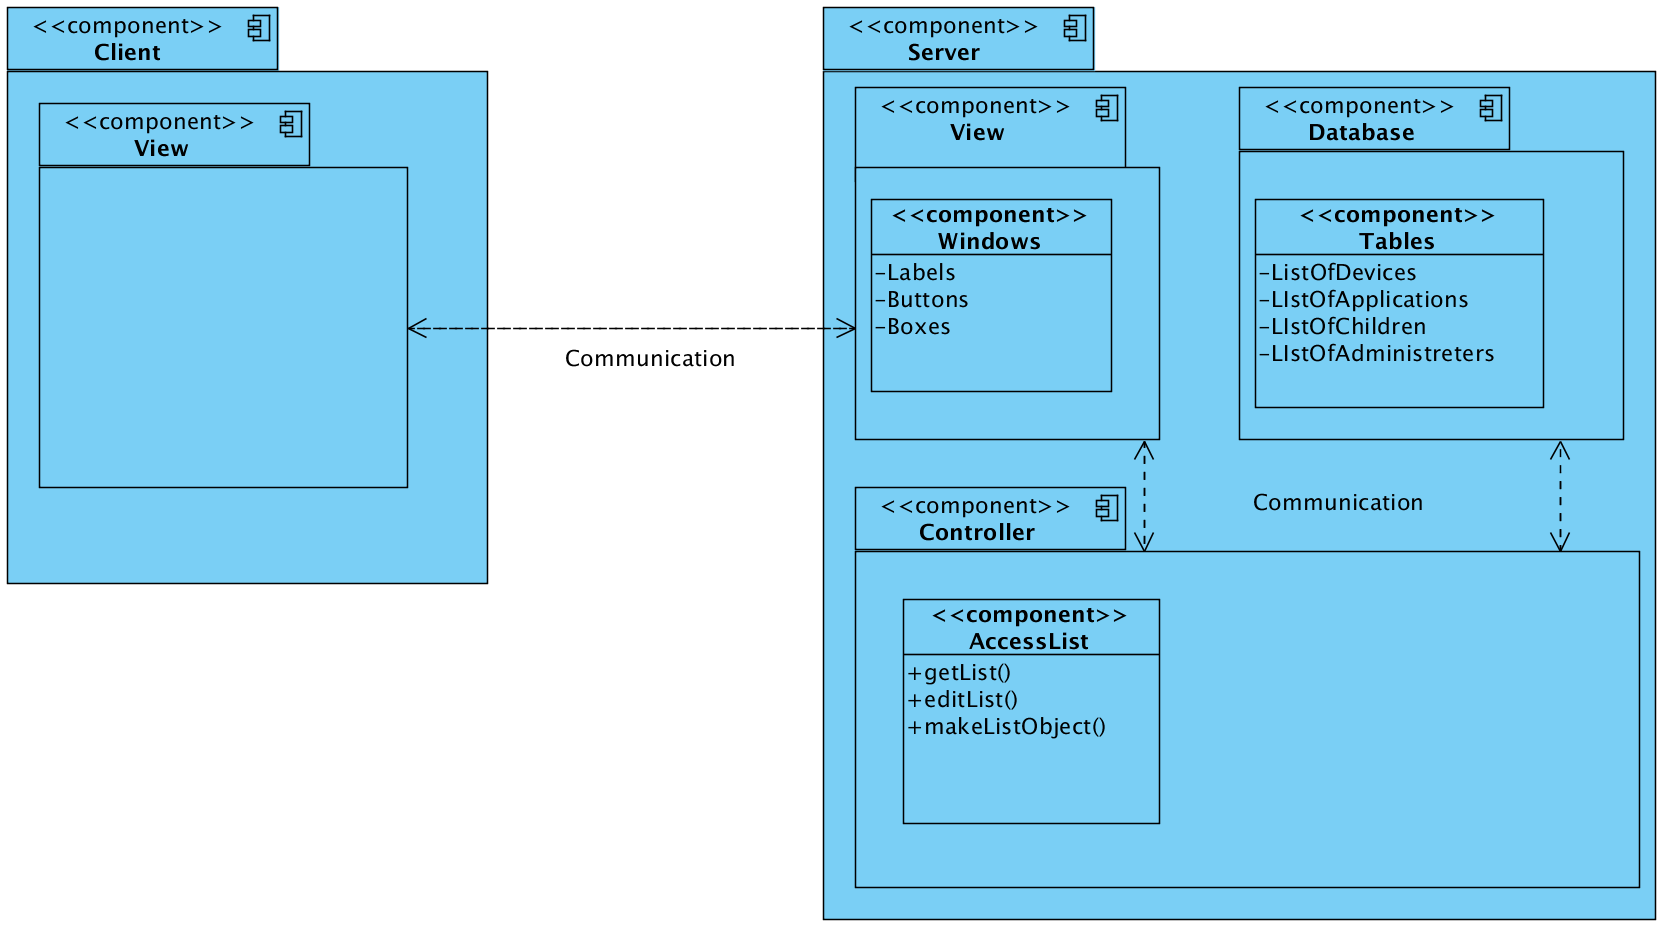
\includegraphics[width=1.0\textwidth]{img/ComponentArketektur.png}
\caption{The figure shows the component architecture of the administrations system}
\label{fig:architecture}
\end{figure}

The three components contain other components, which contain some attributes. These attributes define what function the overall component has, for example the view component contains a windows component, which contains some attributes called ``labels'', ``buttons'' and ``boxes''. The attributes show that the windows component can contain labels, buttons and boxes.
The controller contains a component with an attribute called accesList, this attribute can get a list from the database, edit a list from the database and make an object of a list.
The database contains a component called lists, this component has an attribute which indicates that the database contains lists. Among the lists is a list of devices.